      
               
                \begin{ledgroupsized}[r]{120mm}
                \footnotesize 
                \pstart                
                \noindent\textbf{\"{U}berlieferung:}   
                \pend
                \end{ledgroupsized}
            
              
                            \begin{ledgroupsized}[r]{114mm}
                            \footnotesize 
                            \pstart \parindent -6mm
                            \makebox[6mm][l]{\textit{L}}Konzept: LH XXXVII 3 Bl. 113\textendash114. 1 Bog. 2\textsuperscript{o}. 4 S. zweispaltig. Linke Spalte fortlaufender Text, rechte Spalte Erg\"{a}nzungen und Textkorrekturen. Auf Bl. 113~r\textsuperscript{o} obere H\"{a}lfte rechts drei Zeichnungen. Auf Bl. 113~v\textsuperscript{o} zwei Zeichnungen rechts in der Mitte. Auf Bl. 114 v\textsuperscript{o} obere H\"{a}lfte rechts eine Zeichnung. \\Cc 2, Nr. 487 \pend
                            \end{ledgroupsized}
                %\normalsize
                \vspace*{5mm}
                \begin{ledgroup}
                \footnotesize 
                \pstart
            \noindent\footnotesize{\textbf{Datierungsgr\"{u}nde}: In dem Text werden \"{U}berlegungen des vorausgehenden St\"{u}cks N. 42 mit dem Ziel weitergef\"{u}hrt, zu allgemeing\"{u}ltigen Regeln in Bezug auf das Verhalten elastischer K\"{o}rper zu gelangen. Auch hier sind es Experimente, aus denen Leibniz die Geltung einer Propositio erschließt. Aufgrund der \"{U}bereinstimmung der Wasserzeichen unseres St\"{u}ckes mit N. 42 gehen wir von demselben Entstehungszeitraum aus.}
                \pend
                \end{ledgroup}
            
                \vspace*{8mm}
                \pstart 
                \normalsize
   [113 r\textsuperscript{o}] \textso{Experim. 1.} Si duo Elastica\protect\index{Sachverzeichnis}{elasticum} \edtext{diversarum virium ab eadem}{\lemma{Elastica}\Afootnote{ \textit{ (1) }\ eadem vi eandem \textit{ (2) }\ diversarum virium ab eadem \textit{ L}}} potentia  (tendente vel comprimente) vim patiantur effectus potentiae \edtext{vim afferentis}{\lemma{}\Afootnote{vim afferentis \textit{ erg.} \textit{ L}}}  erunt ut sunt \edtext{eorum vires}{\lemma{sunt}\Afootnote{ \textit{ (1) }\ spatia  \textit{(a)}\ ab Elasticis\protect\index{Sachverzeichnis}{elasticum|textit} cum vis a \textit{(b)}\ eorum seu \textso{Volumina}  Naturalia \textit{ (2) }\ eorum vires \textit{ L}}} reciproce. \edtext{\textso{Spatia} Elasticorum seu \textso{volumina} \textso{naturalia} voco, quae occupant si vis absit. Experientia hujus theorematis tum hoc modo.}{\lemma{reciproce.}\Afootnote{ \textit{ (1) }\ Experientia hujus theorematis commodissime fiet in Elastico\protect\index{Sachverzeichnis}{elasticum|textit} liquido, quale est aer \textit{ (2) }\ Sunto \textit{ (3) }\ \textso{Spatia} Elasticorum   \textbar\ seu \textso{volumina} \textit{ erg.}\ \textbar\ \textso{naturalia} [...] tum \textit{(a)}\ in liquido tum in solido Elastico\protect\index{Sachverzeichnis}{elasticum|textit} fieri potest \textit{(b)}\ in  \textit{(aa)}\ liquido \textit{(bb)}\ solido hoc \textit{(c)}\ hoc modo. \textit{ L}}} Esto lamina ferrea Elastica\protect\index{Sachverzeichnis}{elasticum}  restitutione sua circumagens rotam \edtext{dentatam}{\lemma{}\Afootnote{dentatam \textit{ erg.} \textit{ L}}} \textit{a} elevansque \edtext{pondus columnae dentatae}{\lemma{elevansque}\Afootnote{ \textit{ (1) }\ columnam dentatam \textit{ (2) }\ pondus columnae dentatae \textit{ L}}} \edtext{\textit{bc}. }{\lemma{\textit{bc}}\Afootnote{ \textbar\ usque ad \textit{d} \textit{ gestr.}~\textbar\ . Esto \textit{ L}}}% \begin{wrapfigure}{l}{0.3\textwidth}                    
                %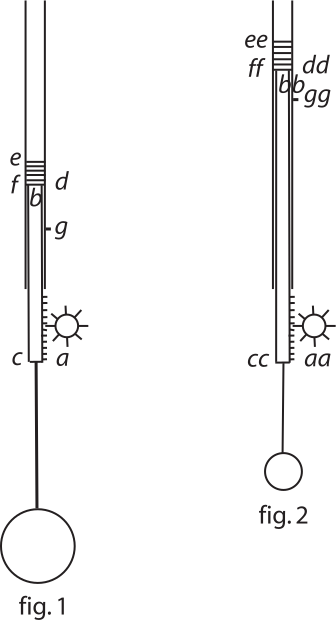
\includegraphics[width=0.3\textwidth]{../images/37_4_113r}
                        %\caption{Bildbeschreibung}
                        %\end{wrapfigure}
                        %@ @ @ Dies ist eine Abstandszeile - fuer den Fall, dass mehrere figures hintereinander kommen, ohne dass dazwischen laengerer Text steht. Dies kann zu einer Fahlermeldung fuehren. @ @ @ \\
                     Esto alia fortior \edtext{circumagens  rotam \textit{aa} et sustinens columnam graviorem \textit{bbcc}}{\lemma{fortior}\Afootnote{ \textit{ (1) }\ elevans \textit{ (2) }\ \textit{aa} elevan \textit{ (3) }\ circumagens  rotam \textit{aa} et  \textit{(a)}\ elevans columnam \textit{(b)}\ sustinens columnam graviorem \textit{bbcc} \textit{ L}}}. \edtext{Quo}{\lemma{\textit{bbcc}.}\Afootnote{ \textit{ (1) }\   \textbar\ altius \textit{ erg.}\ \textbar\  ad \textit{dd} \textit{ (2) }\ Et esto spatium   \textbar\ naturale \textit{ erg.}\ \textbar\  Elaterii\protect\index{Sachverzeichnis}{elaterium|textit} \textit{a} ad spatium naturale Elaterii\protect\index{Sachverzeichnis}{elaterium|textit} \textit{aa} ut \textit{cd} ad \textit{ccdd} \textit{ (3) }\  Quo \textit{ L}}} facto ad comprimendum denuo elaterium\protect\index{Sachverzeichnis}{elaterium} imponatur \edtext{columnae \textit{cd} pondus \textit{ef} et columnae \textit{ccdd} pondus \textit{eeff}.}{\lemma{imponatur}\Afootnote{ \textit{ (1) }\ utrique columnae \textit{cd} et \textit{cc dd} pondus\protect\index{Sachverzeichnis}{pondus|textit} \textit{ef} vel \textit{eeff} aequale \textit{ (2) }\ columnae [...] \textit{eeff}. \textit{ L}}} \edtext{Ponatur}{\lemma{\textit{eeff.}}\Afootnote{ \textit{ (1) }\ Ajo \textit{ (2) }\ Ponatur \textit{ L}}} pondus\protect\index{Sachverzeichnis}{pondus} \textit{ef} \edtext{columnam \textit{fg} depressurum}{\lemma{\textit{ef}}\Afootnote{ \textit{ (1) }\ descensurum \textit{ (2) }\ columnam   \textbar\ \textit{fg} \textit{ erg.}\ \textbar\  depressurum \textit{ L}}} esse ex \textit{d} in \textit{g} deprimet idem pondus\protect\index{Sachverzeichnis}{pondus} vel ei aequale \textit{eeff}  columnam \textit{bb cc} ex \textit{dd} in \textit{gg}  et lineae \textit{ddgg} per quam depressa est columna major \textit{dd cc} erit tanto minor linea \textit{dg} per quam depressa est columna minor \textit{dc} \edtext{quanto}{\lemma{\textit{dc}}\Afootnote{ \textit{ (1) }\ ut est \textit{ (2) }\ quanto \textit{ L}}} columna ejus est columna alterius major. Ratio est, quia \edtext{data potentia aequali effectus sunt}{\lemma{quia}\Afootnote{ \textit{ (1) }\ effectus omnes sunt \textit{ (2) }\  data potentia aequali effectus sunt \textit{ L}}} ut obstacula, id reciproce\edtext{. Obstacula autem sunt vires contrariae, hoc loco}{\lemma{reciproce}\Afootnote{ \textit{ (1) }\ est hoc loco vires \textit{ (2) }\ . Obstacula [...] loco \textit{ L}}} 
                     \edlabel{elatostart}\edtext{Elateriorum.}{\lemma{Elateriorum}\xxref{elatostart}{elatoend}\Afootnote{ \textit{ (1) }\ \textso{Exp. 2.}  \textit{(a)}\ Potentiae diversae eidem Elaterio\protect\index{Sachverzeichnis}{elaterium|textit} applicatae \textit{(b)}\ Pondera diversa  \textit{(aa)}\ eidem Elaterio\protect\index{Sachverzeichnis}{elaterium|textit} applicata, \textit{(bb)}\ ejusdem crassitiei \textit{(aaa)}\ nunquam ita  descendunt, ut punctum praecise pendeant  ex puncto \textit{(bbb)}\ nunquam descendunt in \textit{(ccc)}\ praecise pendent  \textit{(aaaa)}\ ex puncto suo summo \textit{(bbbb)}\  ex   \textbar\ uno \textit{ erg.}\ \textbar\  puncto   \textbar\ quidam \textit{ erg.}\ \textbar\  summo voluminis Elaterii\protect\index{Sachverzeichnis}{elaterium|textit} naturalis. Ponatur in \textso{fig. 1.} pondus columnae \textit{cb} eousque Elaterium\protect\index{Sachverzeichnis}{elaterium|textit} pressisse,  \textit{(aaaaa)}\ ut \textit{(bbbbb)}\ donec descendere columna potuerit  \textit{(aaaaa-a)}\ eo infra \textit{(bbbbb-b)}\ praecise infra \textit{d}. Dico hoc punctum \textit{d} punctum summum voluminis Elaterii\protect\index{Sachverzeichnis}{elaterium|textit} naturalis, ita ut si restituendo se per lineam \textit{dc} assurgere credatur non sit assurrecturum ultra \textit{d}. Et si columna \textit{bc} nec gravis nec levis esse supponatur, ut si aequalis columnae contrapondio retineatur, columnam non iri elevatam nisi exacte in \textit{c}. Et si columnae \textit{fc} quantumcunque pondus aequalis \textit{(c)}\ Hoc Experimentum verum est in li \textit{ (2) }\ \textso{Exp. 2.} Pondera diversa   \textbar\ homogenea \textit{ erg.}\ \textbar\ ejusdem [...] Elaterium \textit{(a)}\ pondere suo \textit{(b)}\ prementia [...] descendetque, \textit{(aa)}\ dummodo sint \textit{(bb)}\ sine ullo renisu  \textit{(aaa)}\ nec \textit{(bbb)}\ at semper \textit{ L}\protect\rule[0cm]{0,5cm}{0cm}}}
                     \pend
                    %
                      \pstart \textso{Exp. 2.} Pondera diversa homogenea ejusdem  crassitiei,  altitudinis quantaecunque idem Elaterium prementia  puncto suo summo nunquam nec  ultra nec citra punctum quoddam  determinatum consistent.  Ponatur in fig. 1. columnam \textit{fc}  pondere suo eousque pressisse Elaterium \textit{a} donec punctum ejus summum \textit{f}  pervenerit in \textit{d} quod praeterire  nequeat. Ajo pondus quodcunque \textit{ef} superadditum ejusdem crassitiei  altitudinis quantaecunque nunquam  descensurum puncto suo summo \textit{e} ultra \textit{d} et totum \textit{ec} quantumcunque quasi \textit{d} suspensum fore. Quod  ita demonstratur: cum pondus \textit{fe} ex altitudine \textit{dc} sit in aequilibrio\protect\index{Sachverzeichnis}{aequilibrium} cum Elaterio nec ultra descendere  possit, ex hypothesi, ideo ut Elaterii  ita et ponderis omnis vis mutuo periit. Quicquid  ergo addetur, effectum suum libere exercebit, descendetque, sine ullo renisu at\edlabel{elatoend} semper
            %Elatorium-Fussnote war ursprunglich hier
                       \textit{fe} aut aequivalens \edtext{in eadem altitudine crassitieque id est ei simile}{\lemma{}\Afootnote{in [...] simile \textit{ erg.} \textit{ L}}} impedietur a\edlabel{113rdesc}\edlabel{1132desc} descensu.\edtext{}{\lemma{descensu.}\xxref{113rdesc}{113vdesc}\Afootnote{ \textbar\ Quod si vero aequaleat ob crassitiem diversam. \textit{ gestr.}\ \textbar\  %\textso{Exper. 3} 
                       \textit{ (1) }\ \textso{Exp. 3.}  \textit{(a)}\ Ideo generaliter quantaecunque  \textit{(aa)}\ sit crassitiei pondus\protect\index{Sachverzeichnis}{pondus|textit} incumbens \textit{(bb)}\ crassitiei aut altitudinis pondera incumbentia sint  \textit{(aaa)}\ semper manebit in spatio \textit{(bbb)}\ extabit ultra in altitudine quacunque ex \textit{d}  \textit{(aaaa)}\ pondus\protect\index{Sachverzeichnis}{pondus|textit} minus altum \textit{(bbbb)}\ pondus\protect\index{Sachverzeichnis}{pondus|textit} altitudinis minoris  \textit{(aaaaa)}\ praevaleat \textit{(bbbbb)}\ aequivaleat \textit{(b)}\ Quod si vero crassities non sit eadem, aut pondera non sint homogenea, tunc semper manebit supra \textit{c} \textit{ (2) }\  \textso{Exper. 3.} [...] sint, \textit{(a)}\ quantum \textit{(b)}\ semper tantundem  \textit{(aa)}\ inter \textit{(bb)}\ supra quodcunque assumtum descensus pondus\protect\index{Sachverzeichnis}{pondus|textit} \textit{(cc)}\ ponderis [...] \textit{c} \textit{ L}}}
                       \pend \clearpage